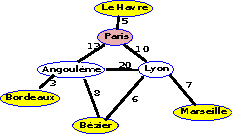
\includegraphics[width=200px]{Images/fig29.pdf}
\titre{Problème du Flot Maximal :} Voici un réseau de transport : \\
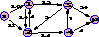
\includegraphics[width=200px]{Images/fig30.pdf}\\
\begin{enumerate}
	\item Un graphe orienté dont les arêtes sont pondérées positivement par une fonction de capacité
	\item Une source à production illimitée
	\item Un puit p à consommation illimitée
\end{enumerate}

\titre{Exemple :}
\begin{enumerate}
	\item boite 1 : $[s,2,4,p]$
	\item boite 2 : $[s,2,1,3,p]$
\end{enumerate}
Une contrainte : Aucune accumulation : ce qui entre est égal à ce qui sort\\
On trouve ici un flot maximal de 23 : \\
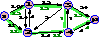
\includegraphics[width=200px]{Images/fig31.pdf}\\

\titre{Méthode pour trouver le flot maximal :} Un flot sur $G$ est une fonction $f$ qui a chaque arc $(u,v)$ associe une quantité $f(u,v)$  telle que :
\begin{enumerate}
	\item $f$ respecte les capacités : $f(u,v) \leq c(u,v)$
	\item Symétrie : $f(u,v) = -f(v,u)$
	\item Conservation du flot : Pour chaque sommet $u$ de $G$ autre que $s$ et $p$ on a $\displaystyle{\sum_{v\in S} = 0}$ (manière formelle de dire : ce qui entre est égal à ce qui sort).
	\item \titre{Flot du réseau :} $F = \displaystyle{\sum_{v\in S} f(s,v)} = \displaystyle{\sum_{v\in S} f(v,p)}$
\end{enumerate}

\titre{Problème du Flot maximal :} Etant donné un réseau de transport $G$, trouver un flot $f$ qui maximise le flot du réseau. \\ 

\titre{Remarque :} Si il y a $m$ sources et $n$ puits, il ne peut y avoir aucune arête qui entre dans une source ou sort d'un puit :\\
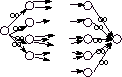
\includegraphics[width=200px]{Images/fig32.pdf}\\

\titre{Annulation des flots}\\
Principe général : \\
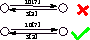
\includegraphics[width=100px]{Images/fig33.pdf}\\
Ajout d'un flux dans le cas de double arête : \\
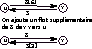
\includegraphics[width=100px]{Images/fig34.pdf}\\
Ajout d'un flux dans le cas d'une simple arête :\\
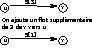
\includegraphics[width=100px]{Images/fig35.pdf}\\

\titre{Réseau résiduel :} Etant donné un réseau de transport $G=(S,A)$, sa fonction de capacité $c$ et un flot $f$ sur $G$. Le réseau résiduel est le même graphe muni de la fonction de capacité $c_f = c(u,v) - f(u,v)$\\

\titre{Exemple :}\\
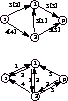
\includegraphics[width=100px]{Images/fig36.pdf}\\

\titre{Remarque :} Soit $f'$ un flot valide sur le graphe résiduel, alors $f+f'$ est un flot valide sur $G$.\\
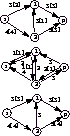
\includegraphics[width=100px]{Images/fig37.pdf}\\
On trace encore le résiduel avec ce nouveau flot : \\
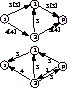
\includegraphics[width=100px]{Images/fig38.pdf}\\

\titre{Propriété :} S'il n'existe aucun chemin de $s$ à $p$ dans le graphe résiduel, alors $f$ est maximal. \\

\titre{Algo de Ford-Fulkerson :} (1954) \\
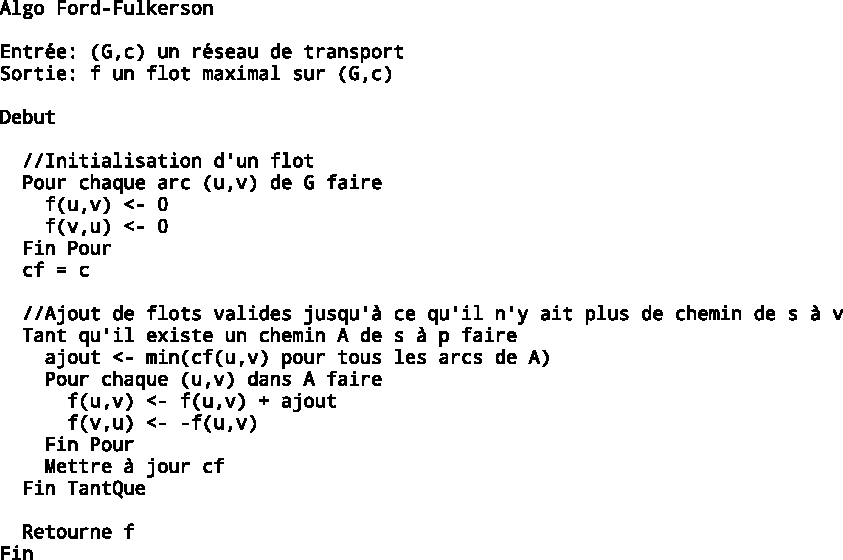
\includegraphics{Images/fig39.pdf}
